\chapter{\label{c:esd-concept}Infrastructure for the control of a plate capacitor electrostatic drive with reduced seismic coupling}
\chaptermark{Infrastructure for the control of a low noise ESD}

\section{Electrostatic drives as actuators in suspended interferometer experiments}
Suspended test masses in interferometers require positional corrections in order for the interferometer to be kept at its operating point. This is typically provided via actuators on the suspension system and predominantly involves voice coil actuators composing magnets and wound wire. Force noise can be introduced to the test masses by their actuators due to various effects such as stray magnetic field coupling, electronic noise in the driver circuitry, Barkhausen noise \cite{Weiss2008} and seismic coupling via the actuator attachment point. The first two effects can usually be mitigated with appropriate design and shielding, for example by choosing appropriate electronic components and by making the magnets small and the electromagnetic environment quiet. The third effect is often mitigated by suspending the actuators from a separate suspension behind the test mass called a \emph{reaction} suspension. This provides seismic filtering to the actuators such that the ground motion coupling introduced to the test masses from the actuators is of similar magnitude to the ground motion the test masses would in any case receive with no actuation.

As introduced in Chapter\,\ref{c:speedmeter-control}, electrostatic drives (\glspl{ESD}) are a type of actuator employed in \GEO{} and \ALIGO{} for fast (high frequency) corrections to the interferometer. This actuator creates a force on a dielectric test mass by creating a potential difference between anodes and cathodes upon the face of the dielectric reaction mass. Electromagnetic field gradients are then formed in such a way that a force can be applied to the test mass in a particular direction.

\subsection{Comb electrostatic drive design}
The \gls{ESD} design used in current generation detectors involves a comb of interlocking anodes and cathodes across which a voltage is applied to create the desired force. Alignment control is achieved through the use of multiple sets of combs on the face of the reaction mass, and the sign of the voltage applied to each set can be controlled to induce torque.

There are a number of problems with this approach actuation. There are obviously cost and technical implications for the use of a reaction suspension system behind each main suspension. The alignment of this second suspension must be controlled and damped in the presence of displacement noise just like the first suspension. With the use of \glspl{ESD}, the gap created between the reaction and test masses can also lead to noise from \emph{squeezed film damping} due to residual gas in the vacuum system \cite{Dolesi2011}. One of the most important issues in the use of this type of \gls{ESD} and the more typical voice coil actuators, however, is the limited clear aperture behind each test mass. In the case of this \gls{ESD} design, the metal comb pattern on its corresponding reaction mass can clip the transmitted beam. The beam size on the \glspl{ETM} of \ALIGO{} is around \SI{6}{\centi\meter} and so in this case if the transmitted light were to be measured for the purposes of sensing and control the choice would have to be made between allowing the beam to be clipped with the associated technical problems this introduces and a reduction in the space available on the reaction mass for the electrostatic comb structure.

\subsection{Plate capacitor electrostatic drive design}
An alternative design to the comb arrangement is to use parallel metal plates with faces perpendicular to the beam axis. Applying a potential difference between these plates effectively creates a capacitor, and the fringe electric field between the edge of the plates and a dielectric test mass produces a small component of force along the beam axis.

The electrostatic energy in the capacitor is given by the volume integral of the electric field created by the potential difference multiplied by the permittivity of the volume enclosed by the plates. For the case when the dielectric mirror is partially inside the volume enclosed by the plates, it can be shown that the energy is given by \cite{Margulies1984}:
\begin{equation}
  E = \frac{1}{2} w d \left( \Delta \phi / d \right)^2 \left( \epsilon z + \epsilon_0 \left( l - z \right) \right),
\end{equation}
where $w$ and $l$ are the plate width and height, respectively, $d$ is the dielectric slab's thickness, $\Delta \phi$ is the potential difference, $\epsilon$ and $\epsilon_0$ are the dielectric and vacuum permittivities and $z$ is the offset of the slab along the beam axis. The electrostatic force the capacitor applies to the dielectric slab in the direction of the beam axis is given by the gradient of the electrostatic energy:
\begin{equation}
  \label{eq:esd-force}
  \begin{split}
    F \left( z \right) &= \nabla E \left( z \right) \\
                       &= \left( \epsilon - \epsilon_0 \right) \frac{w \Delta \phi^2}{2 d}.
  \end{split}
\end{equation}
This shows that the force produced by the parallel plates depends on the voltage applied across the space separating the plates alongside the plate geometry and separation. The force is greater for higher voltage and wider plates with smaller separation.

Originally suggested by Wittel \etal{} \cite{Wittel2015}, this parallel plate capacitor \gls{ESD} has potential applications as an actuator for test masses in suspended interferometers where it was shown that the \gls{DC} force provided by such an actuator with dimensions applicable to the \AEIPROTOTYPE{} is around \SI{1.5}{\micro\newton} at \SI{1}{\kilo\volt}, corresponding to a displacement of around \SI{0.3}{\micro\meter}. This result taken alongside inspection of Equation\,\ref{eq:esd-force} for silica mirrors, feasible plate geometries and voltages shows that this \gls{ESD} design is only suitable for small corrections. As the pendulum systems used in suspended interferometers filter ground motion to a greater extent at higher frequencies, this type of actuation tends to lend itself more to the control of radiation pressure and other displacement effects at frequencies above \SI{50}{\hertz} where seismic motion is typically insignificant.

Apart from the availability of a clear aperture behind the test mass for sensing and control, a further advantage of this type of actuator is that it is highly insusceptible to displacement noise induced by seismic motion; this is due to the shallow gradient of the fringe field at the edge of the plates. Small perturbations with respect to the position of the plates do not strongly couple to the direction or magnitude of the force produced by this type of \gls{ESD}; this contrasts to the seismic noise coupling produced not only by voice coils but also by the metal comb type \gls{ESD}, as shown in \cite{Wittel2015}. The remaining contributions to displacement noise with this type of \gls{ESD} come from misalignments in the plates with respect to one another and electronic noise in the creation of the potential difference across the plates. This chapter will address the design of electronics capable of providing low noise actuation upon the \glspl{ETM} within the \SSMEXPT{}.
% misalignments described by Christian at https://arran.physics.gla.ac.uk/wp/speedmeter/?p=4828

\section{Electrostatic drives for the \SSMEXPT{}}
The plan for the \SSMEXPT{} is to adopt a plate capacitor design for the actuation of the \glspl{ETM} so that the transmitted beam is available for the purposes of sensing and control and to reduce the number of suspensions required in the limited space within the vacuum enclosure.

Due to the dimensions of the \SI{100}{\gram} \glspl{ETM} for which the \glspl{ESD} will eventually be used, the plate capacitor parameters shown in Table\,\ref{tab:ssm-esd-parameters} were deemed appropriate. As Equation\,\ref{eq:esd-force} assumes that the dielectric test mass completely fills the region between the plates it is only an approximation for this situation where each \emph{round} test mass is offset from the plates to avoid ground motion coupling and friction. In order to gain a more complete understanding of the force produced on the test mass by the plates finite element simulations were conducted. A basic model of the plates and test mass described in Table\,\ref{tab:ssm-esd-parameters} was built with \emph{ANSYS} in order to model the effect of force coupling in each direction from an applied voltage, given perfectly aligned plates. Figure\,\ref{fig:ssm-esd-ansys} shows the results of this simulation, with the force along the beam axis given by the z-direction and the forces in the transverse directions given by $x$ and $y$ as a function of potential difference. For a voltage of \SI{750}{\volt}, which is what we think our vacuum feedthrough connectors should be able to handle, the \gls{ESD} is able to provide a force of around \SI{-1.48e-6}{\newton}. The force-voltage behaviour is approximately linear in this region giving a gradient of \SI{-3.68}{\nano\newton\per\volt}.

\begin{table}
  \centering
  \begin{tabular}{ll}
    \textbf{Parameter}   & \textbf{Value} \\
    \gls{ETM} diameter      & \SI{48.6}{\milli\meter} \\
    \gls{ETM} thickness     & \SI{24.5}{\milli\meter} \\
    Single plate width   & \SI{48.6}{\milli\meter} \\
    Single plate length  & \SI{50}{\milli\meter} \\
    Nominal plate separation & \SI{58.6}{\milli\meter} \\
  \end{tabular}
  \caption[Plate capacitor and optic parameters for the \SSMEXPT{}]{\label{tab:ssm-esd-parameters}Plate capacitor and optic parameters for the \SSMEXPT{}.}
\end{table}
% from https://arran.physics.gla.ac.uk/wp/speedmeter/?p=4507

\begin{figure}
  \centering
  \input{graphics/generated/from-python/60-esd-ansys.pgf}
  \caption[Simulations of the actuation force produced by the proposed electrostatic drive design]{\label{fig:ssm-esd-ansys}Simulations of the actuation force produced by the proposed \gls{ESD} design upon a \SI{100}{\gram} cylindrical test mass of diameter \SI{48.6}{\milli\meter} and depth \SI{24.5}{\milli\meter} resembling that of the \SSM{} experiment's \glspl{ETM}. The plate separation and the position of the mirror with respect to the plates influence the level of force produced. Greatest force coupling is produced when the mirror centre of mass is aligned to the edge of the plates and the plates are as close as possible to the mirror without touching. Although the force follows a quadratic relationship with voltage given by Equation\,\ref{eq:esd-force}, the range shown is in a highly linear region.}
\end{figure}

\subsection{Maximum actuation requirements}
At the operating point the \gls{ESD}'s feedback force will be significantly lower than its maximum. The requirement for the \gls{ESD}'s range is set by the lock acquisition sequence performed to reach the low noise state, where the \glspl{ESD} have to be able to respond to changes in classical radiation pressure forces as the light power is increased in the cavities. The suggested lock acquisition schemes for the \SSMEXPT{} require of the order \SI{}{\micro\newton} actuation at high frequencies to bring the test masses to the operating point \cite{Glaefke2015}, and this therefore requires an \gls{HV} amplifier capable of providing close to \SI{750}{\volt} limit set by the vacuum system. The maximum displacement each \gls{ESD} can apply to each \gls{ETM} as a function of frequency given this limit is shown in Figure\,\ref{fig:ssm-etm-disp-esd-max}, calculated using the state-space model for the \glspl{ETM} discussed in Chapter\,\ref{c:speedmeter-control}.

\begin{figure}
  \centering
  \input{graphics/generated/from-python/60-ssm-etm-disp-esd-max.pgf}
  \caption[Maximum end test mass displacement the electrostatic drive can create]{\label{fig:ssm-etm-disp-esd-max}Maximum \gls{ETM} displacement the \gls{ESD} can create as a function of frequency with a potential difference of \SI{750}{\volt}. This is produced by multiplying the force to displacement transfer function calculated for the \glspl{ETM} using a state-space model by the force produced by the \gls{ESD} at maximum output. This assumes that the output is entirely concentrated in a sine wave at each particular frequency, but in reality the feedback signal will contain many frequency components and so the displacement applied at any one frequency will be reduced.}
\end{figure}

Given the experiment's constraints in terms of noise, output voltage and signalling we consider a bespoke \gls{HV} amplifier design. The next sections discuss the design, construction and testing of such a device.

\section{\label{sec:hv-amplifier}High voltage amplifier design and implementation}
Given that there are four \glspl{ETM} in the arm cavities of the \SSMEXPT{} there will be four \glspl{ESD} and so there will need to be four electronic feedback channels. The feedback signal to be applied to each \gls{ESD} via an amplifier will be supplied by the \gls{CDS} system as discussed in Section\,\ref{sec:cds}. Given that a high voltage power supply, safety interlocking and monitoring infrastructure can be shared across the four channels, it is sensible to develop a single electronic amplifier circuit supporting four channels.

\subsection{Differential sending and receiving}
For the control of the amplifier and its high voltage output it is beneficial to utilise \emph{differential} sending and receiving to allow for signals to be transmitted across the laboratory with minimal noise pick-up.

\subsubsection{Control input}
In \gls{CDS}, the signal $S$ is sent from the digital to the analogue domain via \glspl{ADC} where it is split into two channels, $A$ and $B$, containing the same signal but with opposite sign. These signals are sent to the amplifier in a two-core cable, and during transmission the signals are susceptible to noise pick up $n_{A}$ and $n_{B}$, respectively, arising from electromagnetic interference; each channel then contains contributions from the signal and noise:
\begin{align}
  A &= S + n_{A}, \\
  B &= -S + n_{B}.
\end{align}
We can represent these noise sources in terms of common and differential modes at the amplifier input, $n_{\left(+\right)}$ and $n_{\left(-\right)}$, respectively:
\begin{align}
  n_{\left(+\right)} &= n_{A} + n_{B}, \\
  n_{\left(-\right)} &= n_{A} - n_{B}.
\end{align}
Standard op-amps contain \emph{inverting} and \emph{non-inverting} inputs and the output current is proportional to the difference between the two inputs. This subtraction results in the cancellation of common mode noise at the two inputs, so it makes sense to use op-amps to receive the signals sent from \gls{CDS}. An op-amp's ability to remove common mode noise is expressed as its \emph{common mode rejection ratio} (\gls{CMRR}), defined as the logarithm of the ratio of the amplifier's differential and common mode gains $G_{\left( - \right)}$ and $G_{\left( + \right)}$, respectively:
\begin{equation}
  \label{eq:cmrr}
  \text{CMRR} = 20 \log_{10} \left( \frac{G_{\left(-\right)}}{G_{\left(+\right)}} \right),
\end{equation}
with the resulting number expressed in decibels.

The output of an op-amp in terms of its differential and common mode gain is:
\begin{equation}
  S_{\text{out}} = G_{\left(-\right)} \left(A - B\right) + G_{\left(+\right)} \frac{\left(A + B\right)}{2},
\end{equation}
and given the definitions of $A$ and $B$ above, this becomes:
\begin{equation}
  \label{eq:op-amp-common-diff}
  S_{\text{out}} = G_{\left(-\right)} \left(2S + n_{\left(-\right)}\right) + G_{\left(+\right)} \frac{n_{\left(+\right)}}{2}.
\end{equation}
Given Equation\,\ref{eq:cmrr}, an op-amp with high \gls{CMRR} implies $G_{\left(-\right)} \gg G_{\left(+\right)}$, and so Equation\,\ref{eq:op-amp-common-diff} shows that an op-amp with high \gls{CMRR} will result in only differential noise having any significance at the output. The unsuppressed differential noise is kept to a minimum by ensuring that $A$ and $B$ are transmitted through the same shielded cable.

A standard low-noise op-amp such as the OPA277 provides \gls{CMRR} of \SI{120}{\deci\bel} at \SI{100}{\hertz}; this would result in $n_{\left(+\right)}$ being suppressed by a factor $10^6$ which should be sufficient for a standard laboratory environment.

\subsubsection{High voltage output}
Only the potential difference between the plates of each \gls{ESD} determines its force actuation, not the magnitude of the voltage with respect to ground at any one plate. To suppress the effect of noise from the op-amps used to produce the high voltage signals, however, it is best to create the potential difference $V$ by producing balanced contributions of $\frac{V}{2}$ at the cathode and $\frac{-V}{2}$ at the anode. This is to reduce the effect of current noise, which depends on the output voltage, from the \gls{HV} op-amp used to generate the signal. The noise from identical \gls{HV} op-amps is then suppressed by a factor $\sqrt{2}$ between the plates. This requires two \gls{HV} op-amps per output channel.

\subsection{Switchable dewhitening}
During lock acquisition the majority of the \gls{ESD}'s signal will contain corrections for low frequency oscillations created by seismic noise and radiation pressure effects in order to damp the residual test mass motion to the required level. As the operating point is neared the signal will have to contain feedback at higher frequencies to reduce the displacement noise sources shown in Table\,\ref{tab:noise-categories} to reach the target sensitivity.

Whitening and dewhitening was introduced in Section\,\ref{sec:whitening-dewhitening}. To achieve strong actuation at low frequencies during lock acquisition the input to the \gls{HV} amplifier from \gls{CDS} will be unwhitened to achieve maximum low frequency signals at the expense of higher frequency noise from the \glspl{DAC}. When low frequency noise is suppressed and greater locking precision is desired in order to reach the low noise operating point, a whitening filter on \gls{CDS} will be engaged to enhance the higher frequency feedback above the \gls{DAC} noise. To compensate for this digital filter an equivalent dewhitening filter will be required on each analogue \gls{HV} channel as shown in Figure\,\ref{fig:ssm-control-loop-mixed}. For maximum flexibility we intend to include two dewhitening filters for each \gls{HV} channel, and due to the speed at which the control system will have to respond to high frequency perturbations these filters will have to be switchable by an electronic means.

The simulations conducted in Chapter\,\ref{c:speedmeter-control} suggest that the whitening at the output from \gls{CDS} should provide amplification by a factor of \num{10} above \SI{100}{\hertz}, which means the dewhitening should reduce the magnitude by the same amount. Simulating one or two \SI{10}{\deci\bel} active dewhitening circuits as shown in Figure\,\ref{fig:hv-amp-dewhitening-circuit} with the circuit simulation tool \emph{\gls{LISO}} the resulting transfer functions are shown in Figure\,\ref{fig:hv-amp-dewhitening-sims}. The difference in phase between the two filters can be compensated with a sign flip applied to the feedback signal during filter transitions.

\begin{figure}
  \centering
  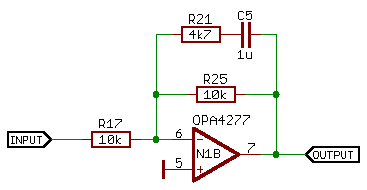
\includegraphics[width=0.6\columnwidth]{graphics/60-hv-amp-dewhitening.pdf}
  \caption[Active inverting dewhitening circuit]{Active inverting dewhitening circuit. This filter uses an inverting op-amp with parallel feedback resistors to achieve the desired frequency response. At low frequencies, the capacitor's impedance is high and so the feedback path is dominated by the impedance of the \SI{10}{\kilo\ohm} resistor and the gain is \num{1}. At high frequencies the capacitor produces very low impedance and so the feedback path's total impedance is the equivalent resistance of the parallel \SI{4.7}{\kilo\ohm} and \SI{10}{\kilo\ohm} resistors and the gain is then $\frac{\SI{10}{\kilo\ohm}}{\SI{3.2}{\kilo\ohm}} \approx \SI{-10}{\deci\bel}$. The simulated transfer functions for one and two of these filters is shown in Figure\,\ref{fig:hv-amp-dewhitening-sims}.}
  \label{fig:hv-amp-dewhitening-circuit}
\end{figure}

\begin{figure}
  \centering
  \input{graphics/generated/from-python/60-hv-amp-dewhitening-sims.pgf}
  \caption[Simulated dewhitening filter frequency response]{Frequency response of the dewhitening filters simulated with \gls{LISO}. Each dewhitening filter provides \SI{-10}{\deci\bel} gain at high frequencies and so the combined pair produces an overall high frequency gain of $\SI{-20}{\deci\bel} \approx \num{e-1}$.}
  \label{fig:hv-amp-dewhitening-sims}
\end{figure}

\subsubsection{Digital switching electronics}
A series of digital outputs from \gls{CDS} can be used to control the \gls{HV} amplifier's dewhitening filters. The Contec DO-32L-PE output card provides a 32 channel binary switch with an equivalent schematic shown in the left side of Figure\,\ref{fig:hv-amp-sigital-switching}. The control signal from \gls{CDS} for a particular output is inverted and attaches to the negative input of an optocoupler which acts as a relay without an electrical connection between the input and output. The positive input is attached to a voltage supply such that a digital output of \num{1} results in a closed circuit once inverted. An output of \num{0} is inverted to \num{1} and so there is no potential difference to close the optocoupler's circuit. The optocoupler's output in turn connects to the base of a transistor which controls current flow between the collector and emitter. Once the potential difference between the transistor's base and emitter exceeds around \SI{0.7}{\volt}, current is allowed to flow from the collector to the emitter, forcing the potential difference between collector and emitter to be zero.

\begin{figure}
  \centering
  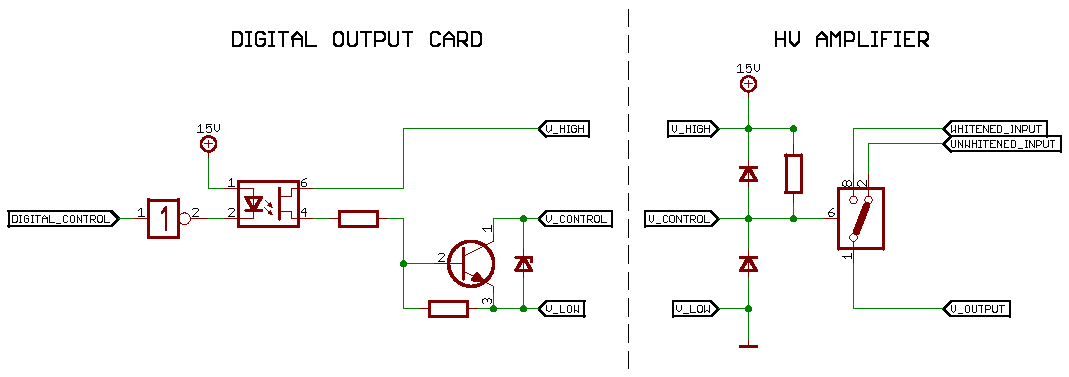
\includegraphics[width=\columnwidth]{graphics/60-hv-amp-digital-switching.pdf}
  \caption[Digital signalling between the control and data acquisition system and a channel within the high voltage amplifier]{\label{fig:hv-amp-sigital-switching}Digital signalling between \gls{CDS} and a channel within the \gls{HV} amplifier. The digital control signal operates an optocoupler which allows current to flow from the $V_{\text{HIGH}}$ voltage reference to a transistor which operates the analogue control signal $V_{\text{CONTROL}}$. This signal is used by the \gls{CMOS} switch in the \gls{HV} amplifier to select either the dewhitened or unfiltered inputs.}
\end{figure}

The analogue input to the \gls{HV} amplifier for a particular channel is split into two with one passed through the dewhitening filter and the other passed through unfiltered. These two signals, the ``dewhitened'' and ``normal'' inputs, respectively, as shown in Figure\,\ref{fig:hv-amp-sigital-switching}, form the poles of a \emph{complementary metal-oxide semiconductor} (\gls{CMOS}) switch, selected for its rapid switching speed. The analogue output from this switch is either the dewhitened or normal input, as determined by a threshold sensor at the switch's control input. If the control voltage is near to \SI{15}{\volt} the output is the dewhitened input, and if it is near to ground the output is the normal input. The voltage drop across the \gls{CMOS} is negligible. The switch control input is connected to one of the digital outputs of the \gls{CDS} card via a shielded transmission line, represented by the dashed vertical line. Also transmitted between the circuits are the reference voltages $V_{\text{HIGH}}$ and $V_{\text{LOW}}$, set to \SI{15}{\volt} and ground, respectively. The software on \gls{CDS} determines whether the control voltage is set to $V_{\text{HIGH}}$ or $V_{\text{LOW}}$. Due to the \emph{active low} operation of the digital output card, where the application of a current to the optocoupler's \gls{LED} (corresponding to a digital control input of \num{1}) results in the control voltage becoming $V_{\text{LOW}}$, the dewhitening filter threshold signal $V_{\text{CONTROL}}$ must be referenced to $V_{\text{HIGH}}$. This is achieved in the circuit through the use of a pull-up resistor. When dewhitening is desired, an output of \num{1} at the optocoupler results in a low-resistance path between the control signal and ground and so the control signal within the amplifier becomes $V_{\text{LOW}}$. A truth table for the logic between \gls{CDS} and the \gls{HV} amplifier is shown in Table\,\ref{tab:digital-dewhitening-truth-table}.

\begin{table}
  \centering
  {\renewcommand{\arraystretch}{1.2} % for extra vertical spacing between rows
    \begin{tabular}{c|c|c}
      \textbf{\gls{CDS} software logic level} & \textbf{$V_{\text{CONTROL}}$} & \textbf{Dewhitening status} \\
      \hline
      0 & $V_{\text{HIGH}}$ & On \\
      1 & $V_{\text{LOW}}$ & Off
    \end{tabular}
  }
  \caption[Truth table for digital switching of dewhitening filters in the high voltage amplifier]{\label{tab:digital-dewhitening-truth-table}Truth table for digital switching of dewhitening filters in the \gls{HV} amplifier, showing the effect that a software logic level in \gls{CDS} has on the dewhitening of the input signal for a particular channel in the \gls{HV} amplifier.}
\end{table}

The electronics shown in Figure\,\ref{fig:hv-amp-sigital-switching} are for a single dewhitener. This configuration must be repeated twice for each of the channels in order to provide available dewhitening of \SI{0}{\deci\bel}, \SI{10}{\deci\bel} or \SI{20}{\decibel}.

\subsection{Choice of high voltage op-amp}
Due to the nature of the load the amplifier does not need to drive a significant current, but the voltage noise it produces must be significantly lower than the displacement requirement for the experiment in order for it not to limit its sensitivity. The lowest noise high voltage amplifier integrated circuits available tend to be \gls{MOSFET}-type op-amps. The choice of device tends to be motivated by the bandwidth, maximum output voltage and noise of each particular model.

The \emph{gain-bandwidth product} specifies an op-amp's open-loop gain as a function of the bandwidth it is able to provide it over, and this figure is derived from the speed at which the op-amp's output is able to react to a change in its input (its \emph{slew rate}). The full output voltage is not provided at the unity gain frequency, however, and so a more useful figure of merit is the bandwidth over which the maximum output can be provided. For the \SSMEXPT{} it is expected that radiation pressure and thermal noise will require fast corrections in the \SI{}{\kilo\hertz} range, and to avoid becoming limited by the device's slew rate at higher frequencies (which appears as phase lag on a plot of the frequency response) it is reasonable to require a bandwidth of at least \SI{20}{\kilo\hertz}.

The required \gls{DC} op-amp gain should be known ahead of time in order to fully estimate the effect an op-amp's noise will have on the experiment. The maximum \gls{CDS} input voltage is \SI{\pm10}{\volt} (differential) and so to achieve the maximum output voltage requirement of \SI{\pm350}{\volt} with the greatest dynamic range the amplifier circuit's gain should be at least $\frac{\SI{\pm10}{\volt}}{\SI{\pm350}{\volt}} = \num{\pm35}$.

Finally, the quiescent current drawn by each op-amp determines the amount of heat it will produce, and since the \gls{HV} amplifier will be used continuously during interferometer operation this parameter should be as low as practical in the chosen model.

Table\,\ref{tab:hv-op-amp-comparison} shows the aforementioned parameters for some popular op-amp models produced by \emph{Apex}. The models shown have sufficient output voltage and identical input noise. The PA89's bandwidth is limited and the full output voltage is not available beyond \SI{7}{\kilo\hertz}, whilst the quiescent power in the PA94 and PA98 is high enough to warrant challenging heat sink requirements. In this case the optimal choice of op-amp is the PA95, which provides enough bandwidth and for which only a passive heat sink will be required.

\begin{table}
  \centering
  \begin{tabular}{r|c|c|c|c}
    & \textbf{PA89} & \textbf{PA94} & \textbf{PA95} & \textbf{PA98} \\
    \hline
    \textbf{Maximum output} & \SI{1140}{\volt} & \multicolumn{2}{c|}{\SI{900}{\volt}} & \SI{450}{\volt} \\
    \textbf{Bandwidth @ \SI{400}{\volt} output} & \SI{7}{\kilo\hertz} & \SI{90}{\kilo\hertz} & \SI{30}{\kilo\hertz} & \SI{60}{\kilo\hertz} \\
    \textbf{Input noise @ \SI{100}{\hertz}} & \multicolumn{4}{c}{\SI{6}{\nano\volt\per\sqrthz}} \\
    \textbf{Quiescent power @ \SI{\pm400}{\volt}} & \SI{3.8}{\watt} & \SI{14.1}{\watt} & \SI{1.3}{\watt} & \SI{17.5}{\watt}
  \end{tabular}
  \caption[Performance specifications for various high voltage operational amplifiers]{\label{tab:hv-op-amp-comparison}Performance specifications for various \gls{HV} op-amps. All of the models listed are manufactured by Apex and the values have been obtained from their respective data sheets. The PA95 was selected due to its low quiescent power for the desired voltage range, which in turn eases the requirement for heat sinking, and the bandwidth is sufficient for the \SSMEXPT{}.}
\end{table}

\subsection{Amplifier signal path}
The constructed amplifier signal path is shown for a single channel in Figure\,\ref{fig:hv-amp-signal-path}. The inputs IN+ and IN- are differentially received and converted to a single-ended signal which is then passed through the two dewhitening stages controlled by digital switches. The signal is then split into two parts, with one part being inverted, and these become the inputs to the PA95 \gls{HV} op-amps. The inverting and non-inverting inputs on each op-amp are bridged with diodes to ensure that the voltage difference is less than \SI{\pm0.7}{\volt}; this is to prevent accidental overvoltage at the inputs. Although the differential input range of the PA95s is \SI{\pm20}{\volt}, the \SI{\pm0.7}{\volt} limit is sufficient to reach the required bandwidth in this application, and avoids potential damage to the costly op-amps from incorrect input. A \SI{1}{\percent} voltage divider at each of the differential outputs provides a signal that is within the input range of \gls{CDS} for the purpose of output monitoring. This so-called \emph{monitor} provides a reference channel for the controller in order to assist with the calibration of the device as well as a possible error signal extraction point for a feedback loop intended to suppress amplifier noise. The resistors near pins 7 and 8 of each op-amp provide current limiting, discussed in Section\,\ref{sec:hv-amp-current-limit}. The capacitor placed between pins 4 and 6 on each amplifier provides compensation for the phase of the op-amp at high frequencies, and its value is determined from a look-up table provided by the manufacturer.

\begin{figure}
  \centering
  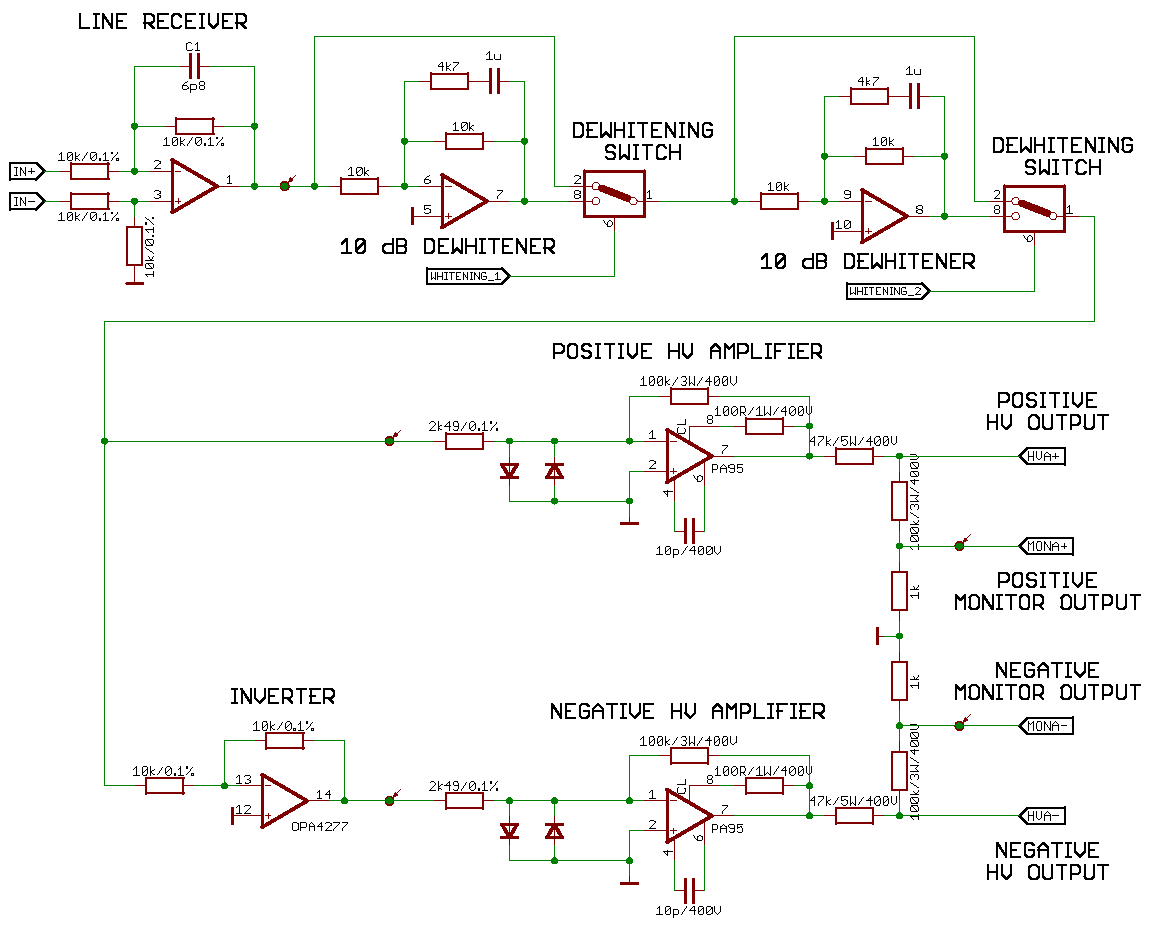
\includegraphics[width=\columnwidth]{graphics/60-hv-amp-signal-path.pdf}
  \caption[High voltage amplifier signal schematic]{\label{fig:hv-amp-signal-path}Schematic of a single high voltage amplifier channel. The input from \gls{CDS} is differentially received, dewhitened and then split into differential outputs that are amplified by PA95 op-amps. A pick-off reads \SI{1}{\percent} of the output voltage for calibration and noise projection purposes.}
\end{figure}

\subsection{Practical and safety features}
As the \gls{HV} amplifier handles potentially lethal current and voltage, a number of additional features beyond the signal circuitry are present.

\subsubsection{\label{sec:hv-amp-current-limit}Current limiting}
At the output of each \gls{HV} rail there are \SI{47}{\kilo\ohm} series resistors which passively limit the current on each rail to around \SI{10}{\milli\ampere}. The current limit does not impact the driving of capacitive loads, but ensures that the current produced by the \gls{HV} amplifier is not lethal. Given this series resistance the \gls{HV} transmission lines to the vacuum system must be kept short ($<\SI{3}{\meter}$) to prevent capacitance in the cable from creating a low-pass response within the bandwidth of the experiment.

The resistor placed between pins 7 and 8 also acts as an \emph{active} current limit. The voltage drop across this resistor is used by each PA95 to limit its output current. The combination of the two current limiting features ensures that a single fault will not lead to lethal output current, and as such this feature of the circuit meets European standard EN\,61010 \cite{EN2010}.

\subsubsection{Soft-start}
Capacitors are present upon the \gls{HV} supply lines to filter \gls{AC} noise, and these must be charged when the device is switched on. Normally these capacitors would present very little impedance to the power supplies and so a large initial current would be drawn potentially damaging components in its path. The simplest technique to prevent this from happening would be to put resistors in the path of the power supplies, but resistors that would charge the capacitors at a safe rate in a short time would also dissipate a lot of power and require additional heat sinking. Instead, we use a \emph{soft-start} mechanism which controls the current flow during the charging of the capacitors. The \gls{HV} amplifier's on-off switch operates optocouplers which allow current to flow into the circuit. Initially, when the circuit's \gls{HV} capacitors are discharged, the current on each \gls{HV} rail is limited by the parallel \SI{5}{\kilo\ohm} resistors. A \SI{2.5}{\percent} pick-off from each \gls{HV} rail is compared to a reference \SI{5}{\volt} potential at an op-amp, the output of which operates a second optocoupler on each rail. When the voltage surpasses \SI{200}{\volt} the power the \SI{5}{\kilo\ohm} resistors dissipate is \SI{8}{\watt}, which is near their limit. At this point, the capacitors are almost fully charged and the pick-off voltage surpasses the \SI{5}{\volt} reference and so the op-amp's output operates the optocoupler to open up a low-resistance path that bypasses the \SI{5}{\kilo\ohm} resistors and prevents them from overheating. The soft-start circuit is shown in Figure\,\ref{fig:hv-amp-soft-start}. The capacitors to be charged by this circuit would be attached between the +HV and -HV rails and ground.

\begin{sidewaysfigure}
  \centering
  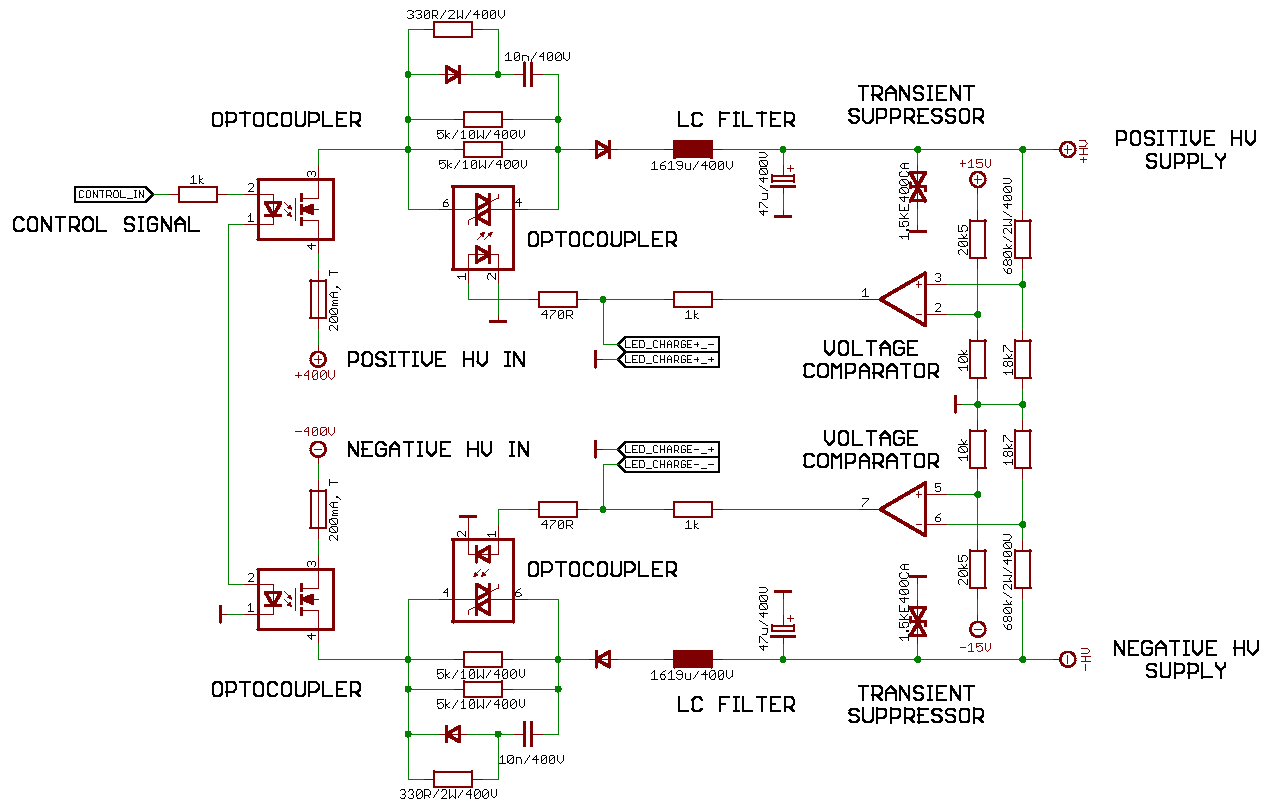
\includegraphics[width=0.75\columnwidth]{graphics/60-hv-amp-soft-start.pdf}
  \caption[High voltage amplifier soft-start schematic]{\label{fig:hv-amp-soft-start}Soft-start mechanism to prevent excessive power supply current draw. This is based on a design for the \AEIPROTOTYPE{} by Andreas Weidner. The leftmost optocouplers control whether current is allowed to flow from the power supplies given a control signal from an on-off switch on the enclosure. After the electronics are switched on, the current flow is initially limited by two \SI{5}{\kilo\ohm} resistors. Any \gls{AC} signal content above around \SI{500}{\hertz} is filtered by the presence of an low-pass LC filter formed of the \SI{1619}{\micro\henry} choke and \SI{47}{\micro\farad} capacitor (the low-pass corner frequency decreases further when additional capacitive load is attached). A \SI{2.5}{\percent} pick-off from each \gls{HV} rail is compared to a \SI{\pm5}{\volt} reference, with the resulting difference fed back to a second pair of optocouplers (different models from the first due to their lower duty cycle) which gradually open up a low-resistance path on each supply rail. Without these optocouplers, the power the \SI{5}{\kilo\ohm} resistors would need to dissipate would be considerable at maximum voltage. As the supply voltage increases beyond around \SI{200}{\volt}, the resistance through the optocoupler is reduced far below the \SI{5}{\kilo\ohm} resistors and so the power dissipated in the resistors is negligible.}
\end{sidewaysfigure}

\subsubsection{Pressure and temperature interlock}
The breakdown voltage of the plate capacitors as a function of pressure, given by Paschen's Law, has a minimum in the region of \SI{e-1}{\milli\bar} to \SI{e1}{\milli\bar} depending on the separation and geometry of the anode and cathode. If the gas pressure and plate separation are favourable, it is possible for arcing to occur between the anode and cathode of each \gls{ESD}. Estimates of the Paschen curves for parallel plates with varying separations in nitrogen are shown as a function of pressure in Figure\,\ref{fig:esd-paschen}. Apart from arcing, related effects such as creepage\textemdash tracking of charge across insulative surfaces\textemdash can lead to arcing at voltages above \SI{50}{\volt} in low vacuum, though the use of highly insulating material such as ceramics can help to mitigate this risk almost entirely \cite{EN2010}.

Although the use of high voltage plate capacitors is in general safe at both atmospheric pressure and high vacuum, the act of pumping gas out of the vacuum system passes through pressures at which arcing and surface tracking can occur. To prevent this possibility a cut-off function was implemented within the circuit to prevent \gls{HV} output unless a control signal is supplied (see Figure\,\ref{fig:hv-amp-interlock}). The switching mechanism uses the same \gls{CMOS} switches as the digital dewhitening filters shown in Figure\,\ref{fig:hv-amp-sigital-switching}, with the threshold signal being generated by \gls{CDS} based on a signal from a separate pressure monitor input. Additionally, as a temperature fail-safe for the amplifier components, temperature sensors are present within the enclosure which operate threshold switches able to remove the supply to the \gls{HV} op-amps using the same mechanism as the pressure interlock. The outputs from each interlock are sent to an AND gate, and only if both the pressure and temperature switches are in a safe state will the \gls{HV} op-amp's supplies switch on. The interlock circuit is shown in Figure\,\ref{fig:hv-amp-interlock}.
% pressure vs voltage claim from speedmeter labbook, at https://arran.physics.gla.ac.uk/wp/speedmeter/2015/01/30/esd-hv-amplifier-pressure-cutoff/

\begin{figure}
  \centering
  \input{graphics/generated/from-python/60-esd-paschen.pgf}
  \caption[Minimum breakdown voltage between the two plates of the electrostatic drive for different separations]{\label{fig:esd-paschen}The minimum breakdown voltage between the two plates of the \gls{ESD} for different separations. This is calculated using Paschen's Law, assuming nitrogen gas and a flat plate geometry. The real effect is a lot more complicated than this model, but the steep slope at lower pressures shown here indicates that the voltage created by the \gls{HV} amplifier for the \glspl{ESD} will avoid problems associated with arcing as long as the vacuum system is operated at atmosphere or high vacuum.}
\end{figure}

\begin{figure}
  \centering
  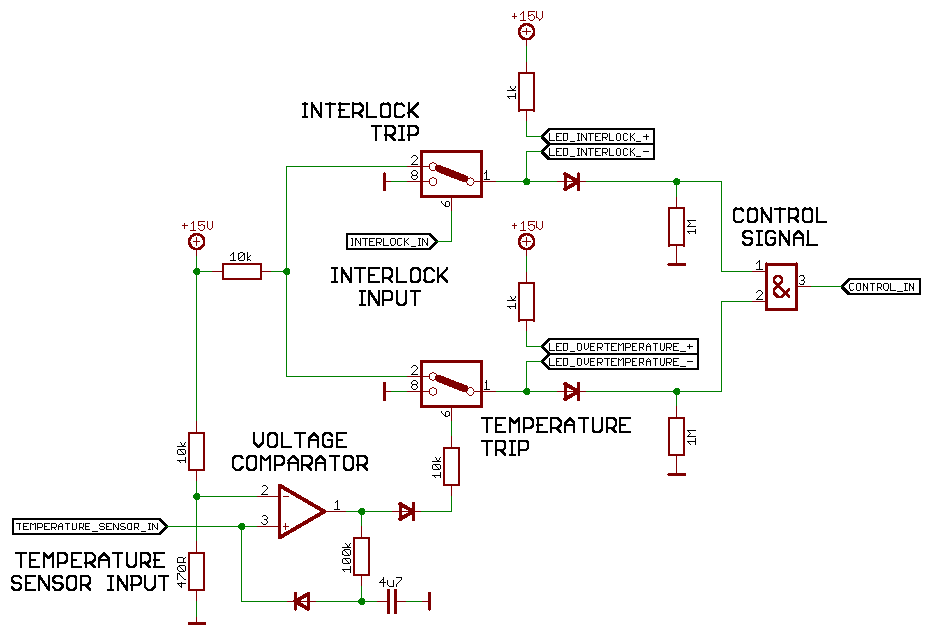
\includegraphics[width=\columnwidth]{graphics/60-hv-amp-interlock.pdf}
  \caption[High voltage amplifier interlock schematic]{\label{fig:hv-amp-interlock}Pressure and temperature interlock circuit. The digital interlock signal from \gls{CDS} operates one switch and the output from a temperature sensor threshold switch operates another. Only if both switches output \SI{15}{\volt} will the control signal used to operate the \gls{HV} supplies switch on.}
\end{figure}

\subsection{Transfer functions and noise measurements}
The monitor output provides a means of measuring \SI{1}{\percent} of the full \gls{HV} output with a signal that is within the input range of \gls{CDS}. This allows transfer functions from the input to the output of each channel to be calculated in software to assist in the eventual calibration of the experiment. The \gls{HV} amplifier should provide gain to the input signal without applying \gls{AC} filtering beyond the desired dewhitening within the intended bandwidth of the experiment. Similarly, the noise measured at the output should not be significant enough to affect the sensitivity of the interferometer by applying force noise to the test masses. The following subsections describe measurements to assert these characteristics.

\subsubsection{Swept sine response of each channel}
Transfer functions for the \gls{HV} amplifier can be measured by injecting a known signal into one channel and measuring the corresponding output. Figure\,\ref{fig:hv-amp-dewhitened-tfs} shows the \emph{swept sine} response, calculated by injecting a sine wave at a given frequency, measuring the output signal and dividing it by the injection, and repeating this process over a given frequency range. These measurements were made without the digital dewhitening switches disengaged such that they provide \SI{20}{\deci\bel} of low-pass filtering. The figure shows the response expected from the predictions made by \gls{LISO} shown in Figure\,\ref{fig:hv-amp-dewhitening-sims}, and the measurements agree once the filtering effect of the \gls{CDS} anti-aliasing filters are taken into account.

\begin{figure}
  \centering
  \input{graphics/generated/from-python/60-hv-amp-dewhitened-tfs.pgf}
  \caption[Frequency response of the high voltage amplifier's channels with dewhitening enabled]{Second amplifier transfer functions with dewhitening enabled. The expected performance of the dewhitening filter from theory is shown in purple alongside the transfer functions of each channel. The curves agree closely, showing that the implemented filter operates as expected. The mismatch at high frequency is caused by the anti-aliasing filters implemented in \gls{CDS}, which aggressively filter signals above a few \SI{}{\kilo\hertz}.}
  \label{fig:hv-amp-dewhitened-tfs}
\end{figure}

\subsubsection{Response with and without dewhitening}
Figure\,\ref{fig:hv-amp-channel-one-tfs} shows swept sine measurements of the first channel with the dewhitening filters in various states: both on, the first on and the second off, the first off and the second on, and both off. The measurements match predictions and the response with both dewhiteners off is flat as intended across the measurement band.

\begin{figure}
  \centering
  \input{graphics/generated/from-python/60-hv-amp-channel-one-tfs.pgf}
  \caption[Transfer functions of the high voltage amplifier input to monitor output with the dewhiteners on and off]{Transfer functions of the high voltage amplifier input to monitor output with the dewhitening filters on and off. The monitor output is a \SI{1}{\percent} pick-off from the main \gls{HV} output, and so the gain is \num{0.4} instead of \num{40}. The curves simulated with \gls{LISO} agree exactly with the measurements within the bandwidth of \gls{CDS}, and at higher frequencies the transfer functions are suppressed by anti-aliasing filters.}
  \label{fig:hv-amp-channel-one-tfs}
\end{figure}

\subsubsection{Coherence between channels}
The channels should be isolated from one another such that a signal injected at one input does not appear at the output of another. Op-amp power supply filtering is implemented using decoupling capacitors, inductors and diodes such that there should be minimal cross-coupling between the channels. Figure\,\ref{fig:hv-amp-coherence} shows the coherence for each channel to each other channel, measuring whether the output signal has the same phase angle as the input signal. Coherence of \num{1} indicates that there is causal coupling between the two channels, whereas coherence less than around \num{0.5} is expected from statistical random noise processes. The results confirm that a high level of isolation between channels has been achieved.

\begin{figure}
  \centering
  \input{graphics/generated/from-python/60-hv-amp-coherence.pgf}
  \caption[High voltage amplifier cross-channel coherence]{\gls{HV} amplifier cross-channel normalised coherence. A swept sine was injected into each channel in turn whilst measurements of the output phase were made on all four channels. In each case, only the channel with the injection has coherence of \num{1}, while other channels only show the effect from noise.}
  \label{fig:hv-amp-coherence}
\end{figure}

\subsubsection{Output voltage noise}
The noise at the output of the first channel of the \gls{HV} amplifier is shown in Figure\,\ref{fig:hv-amp-output-noise}. This was calculated via the \gls{HV} amplifier's monitor with the measured noise being projected into effective \gls{HV} noise by multiplying the signal by the inverse of the monitor pick-off fraction, \num{100}. To measure the noise at frequencies comparable to the \SSMEXPT{}'s cavity bandwidth a Stanford Research SR785 spectrum analyser was used; as shown in Figure\,\ref{fig:aa-ai-filter-tfs} the anti-aliasing and anti-imaging filters significantly reduce the input to and output from \gls{CDS} above \SI{9}{\kilo\hertz} and so they are not practical for this measurement.

The following measurements were made:
\begin{itemize}
  \item the \gls{HV} amplifier's output noise when it is disconnected from \gls{CDS} and has no input signal;
  \item the \gls{HV} amplifier's output noise when it is connected to the \gls{CDS} \glspl{DAC} with an input signal equivalent to maximum \gls{HV} output;
  \item the spectrum analyser noise floor with a \SI{50}{\ohm} load.
\end{itemize}
Each of the spectral densities shown were produced using amplitude spectral density estimates of the time domain signal (see Appendix\,\ref{sec:fourier-transform}), and to avoid windowing effects as discussed in Appendix\,\ref{sec:windowing} the measurements were made with averages across three bands: \SI{250}{\milli\hertz} to \SI{200}{\hertz} (\num{16} averages), \SI{4}{\hertz} to \SI{3.2}{\kilo\hertz} (\num{64} averages) and \SI{128}{\hertz} to \SI{102.4}{\kilo\hertz} (\num{1024} averages). The measured monitor noise is above the input noise of the spectrum analyser in all cases.

The left y-axis shows the measured monitor noise. The right y-axis shows the noise projected into equivalent noise on the \gls{HV} output. The noise is different in the case of zero (orange) or full (green) \gls{DC} output not because of an input voltage dependency but rather due to the inclusion of the \gls{CDS} \glspl{DAC} in the signal path in the latter case which contribute noise as discussed in Section\,\ref{sec:adcs-and-dacs}. Some large amplitude noise is present around \SI{50}{\hertz} and its first harmonic due to pick-up from the electricity mains on the power supply.

\begin{figure}
  \centering
  \input{graphics/generated/from-python/60-hv-amp-output-noise.pgf}
  \caption[High voltage amplifier output noise]{\gls{HV} amplifier output noise. The noise of the amplifier was measured using the monitor output of the first channel, and this is shown in the green and orange traces using the left y-axis. The output noise projected from the monitor to the \gls{HV} rails is shown on the right y-axis. The green trace represents the noise from the amplifier when the input is at maximum and includes the noise contribution from the \glspl{DAC} on \gls{CDS}. The orange trace shows the output noise when \gls{CDS} is not connected. The noise floor of the SR785 spectrum analyser used to make these measurements is shown in blue.}
  \label{fig:hv-amp-output-noise}
\end{figure}

\subsubsection{Effective displacement noise}
As shown in Equation\,\ref{eq:esd-force} the \gls{ESD} force depends on the square of the potential difference. We can rearrange it to show:
\begin{equation}
  \frac{F \left( V_{\text{signal}} \right)}{V_{\text{signal}}^2} = \frac{F \left( V_{\text{signal}} + V_{\text{noise}} \right)}{\left( V_{\text{signal}} + V_{\text{noise}} \right)^2},
\end{equation}
where $V_{\text{noise}}$ is the \gls{HV} amplifier's output noise. This shows that the force noise created by the \gls{HV} amplifier will be greatest at maximum output signal, $V_{\text{signal}} = \SI{750}{\volt}$. The effective force noise is simply the force produced due to the signal subtracted from the total force produced in the presence of signal and noise:
\begin{equation}
  F \left( V_{\text{noise}} \right) = F \left( V_{\text{signal}} + V_{\text{noise}} \right) - F \left( V_{\text{signal}} \right).
\end{equation}

The \gls{ETM} displacement noise this would create is then simply the product of the force noise and the suspension transfer function, and this is shown in Figure\,\ref{fig:hv-amp-output-displacement-noise}. The effective displacement noise is below the noise budget presented in Chapter\,\ref{c:speedmeter-control} within the measurement band, and given that this assumes the \gls{ESD} is at maximum output the displacement noise when the interferometer is at the operating point, requiring only a fraction of its maximum range, will be lower. If the noise from the \gls{HV} amplifier is found to be higher in practice, it should be possible to feed the monitor outputs back to their respective inputs in order to stabilise each channel.
% (Would need to have the whitening calibrated out in real time, but this would be pretty straightforward since the filters are so simple.)

\begin{figure}
  \centering
  \input{graphics/generated/from-python/60-hv-amp-output-displacement-noise.pgf}
  \caption[High voltage amplifier output projected end test mass displacement noise]{\gls{HV} amplifier output voltage noise (without dewhiteners engaged) projected into effective \gls{ETM} displacement noise. The force produced by the \gls{ESD} is a function of the square of the voltage across its plates, and so the noise produced by the \gls{HV} amplifier has greatest effect when the signal is at a maximum. This plot shows the displacement noise for maximum signal, and within the measurement band (blue shaded region) it is below the requirement shown in black taken from the analysis conducted in Chapter\,\ref{c:speedmeter-control}. If necessary the \gls{HV} amplifier's noise could be reduced further by implementing a control loop between its monitor outputs and signal inputs.}
  \label{fig:hv-amp-output-displacement-noise}
\end{figure}

\section{Outlook}
For the control of suspended test masses at high frequencies, parallel plate capacitor \glspl{ESD} provide a low noise alternative to voice coils and their geometry can prevent clipping losses suffered in the use of metal comb \glspl{ESD}. It is intended for parallel plate capacitor \glspl{ESD} to be used as the high frequency actuators in the \SSMEXPT{} presented in Chapter\,\ref{c:speedmeter-intro}, and in order to provide actuation at the required level an \gls{HV} signal with suitably high magnitude and low noise must be available. The technical design of an \gls{HV} amplifier was presented which meets the experiment's range and noise requirements, providing output up to \SI{750}{\volt} with noise of around \SI{20}{\micro\volt\per\sqrthz} in the frequency band of interest.

\begin{sidewaysfigure}
  \centering
  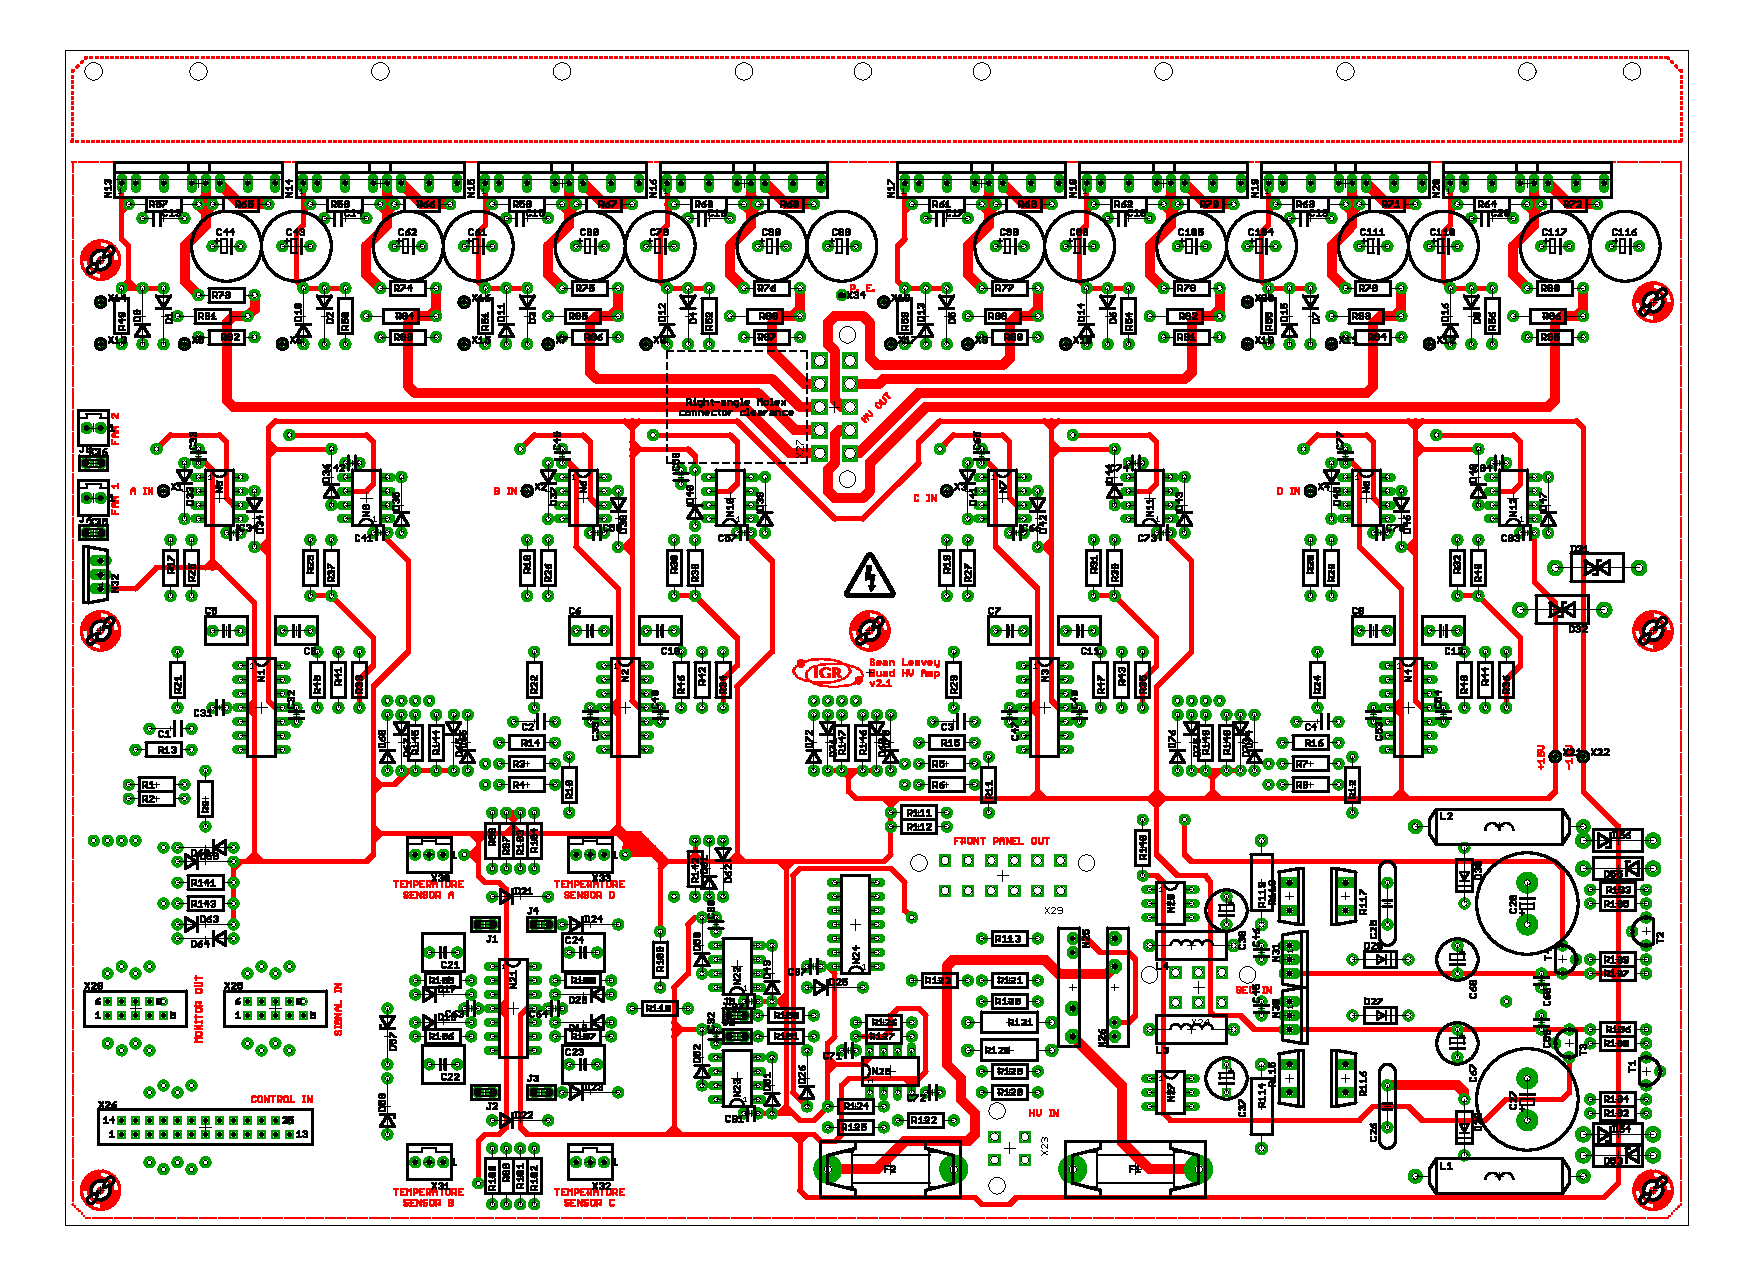
\includegraphics[width=0.8\textwidth]{graphics/60-hv-amp-top.pdf}
  \caption[High voltage amplifier board, top view]{\label{fig:hv-amp-top}Top view of the \gls{HV} amplifier printed circuit board showing the component and copper track layout. This side contains most of the components and all of the connectors that go to and from the enclosure. Areas not carrying signals are part of the ground plane, except for a relief at one side where the heat sinks for the PA95s are attached, isolated from the ground plane to minimise the risk of arcing.}
\end{sidewaysfigure}

\begin{sidewaysfigure}
  \centering
  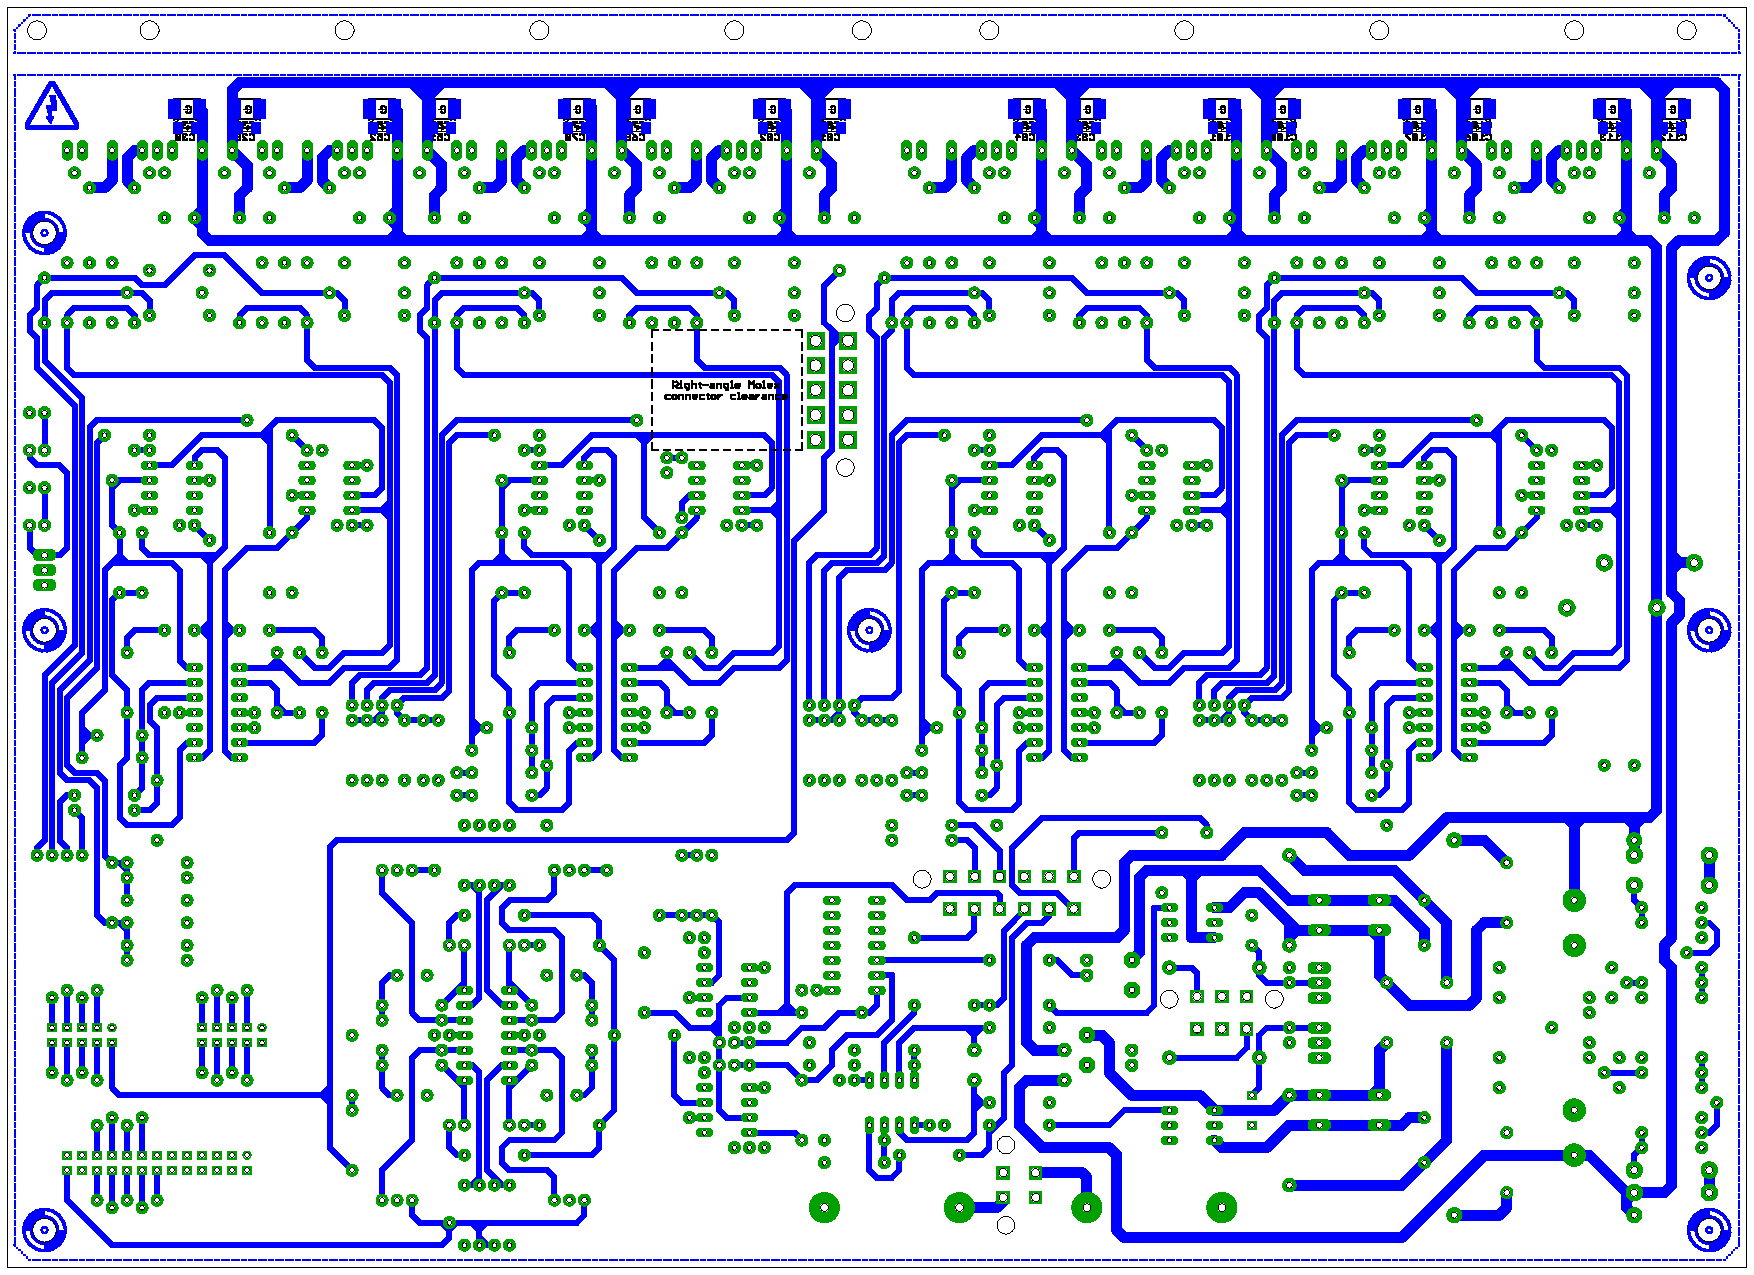
\includegraphics[width=0.8\textwidth]{graphics/60-hv-amp-bottom.pdf}
  \caption[High voltage amplifier board, bottom view]{\label{fig:hv-amp-bottom}Bottom view of the \gls{HV} amplifier printed circuit board showing the component and copper track layout. This side is where the top components are soldered to the copper tracks. Some surface mount decoupling capacitors for the supply rails of the PA95s are present on the bottom as they could not be placed as closely to the op-amps on the top side.}
\end{sidewaysfigure}